\documentclass[conference]{IEEEtran}
\IEEEoverridecommandlockouts
% The preceding line is only needed to identify funding in the first footnote. If that is unneeded, please comment it out.
\usepackage{cite}
\usepackage{amsmath,amssymb,amsfonts}
\usepackage{algorithmic}
\usepackage{graphicx}
\usepackage{textcomp}
\usepackage{xcolor}
\usepackage{float}
\def\BibTeX{{\rm B\kern-.05em{\sc i\kern-.025em b}\kern-.08em
    T\kern-.1667em\lower.7ex\hbox{E}\kern-.125emX}}
\begin{document}

\title{CENG466, Fall 2022, THE 4\\

}

\author{\IEEEauthorblockN{1\textsuperscript{st} Fırat Ağış}
\IEEEauthorblockA{\textit{Department of Computer Engineering} \\
\textit{Middle East Technical University}\\
Ankara, Turkey \\
e2236867@ceng.metu.edu.tr}
\and
\IEEEauthorblockN{2\textsuperscript{nd} Robin Koç}
\IEEEauthorblockA{\textit{Department of Computer Engineering} \\
\textit{Middle East Technical University}\\
Ankara, Turkey \\
e2468718@ceng.metu.edu.tr}
}

\maketitle

\begin{abstract}

\end{abstract}

\begin{IEEEkeywords}

\end{IEEEkeywords}

\section{Object Counting}
    \begin{figure}[h]
        \centering
        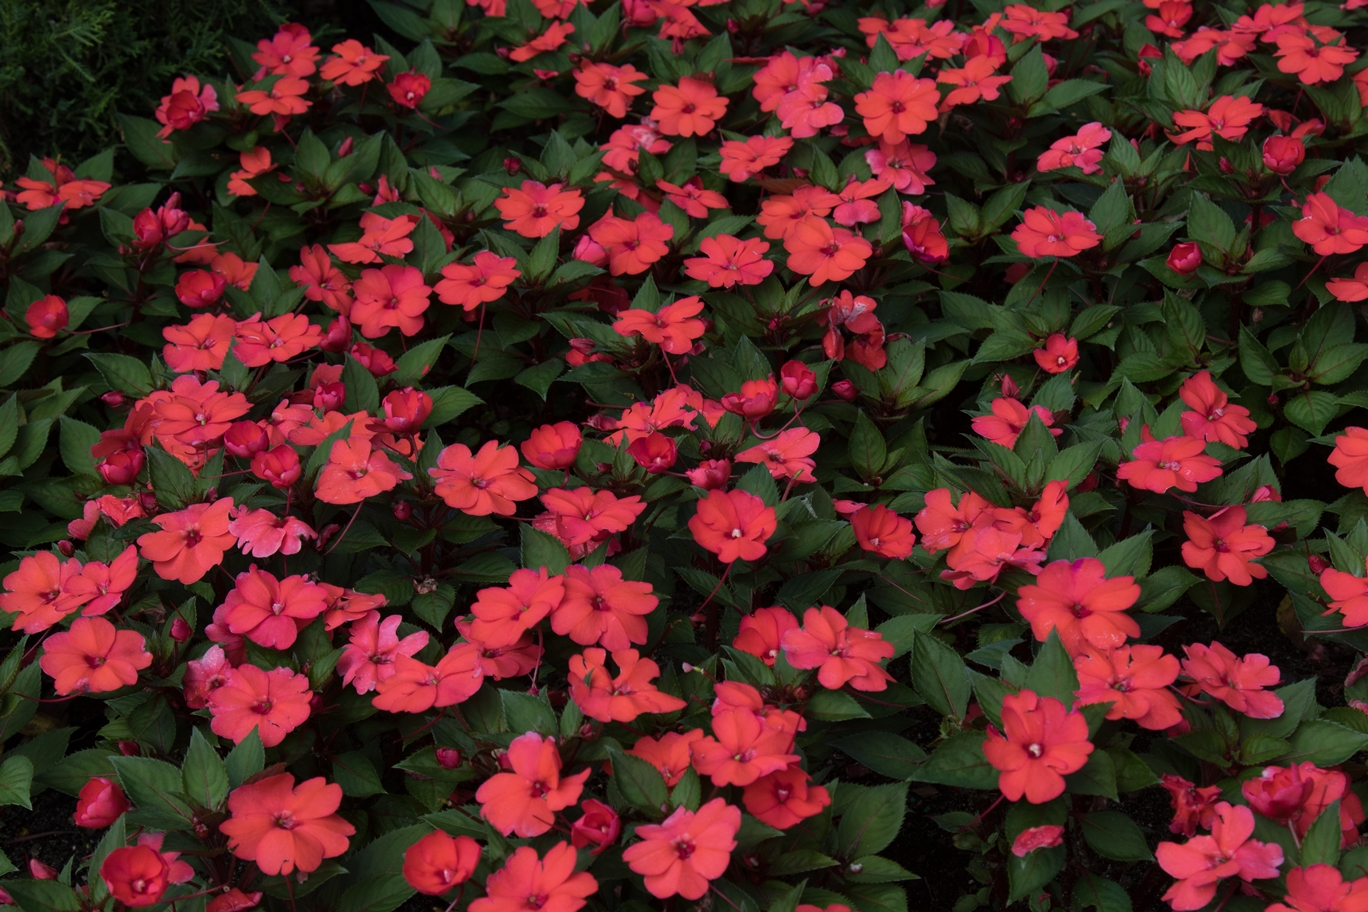
\includegraphics[width=0.4\textwidth]{resources/A1_compact.jpg}
        \caption{Original A1.png}
        \label{fig:a1_input}
    \end{figure}
    \begin{figure}[h]
        \centering
        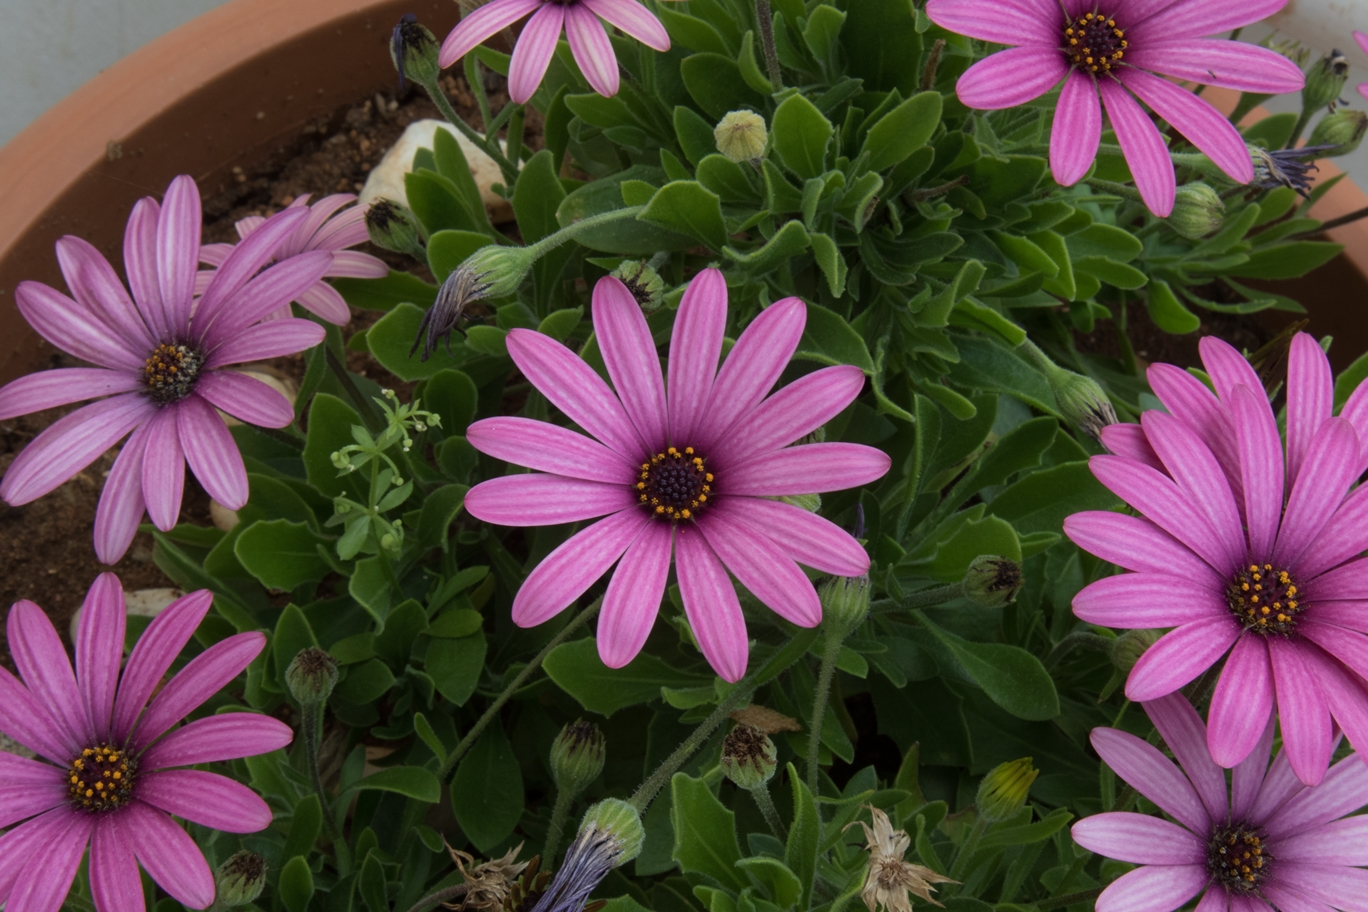
\includegraphics[width=0.4\textwidth]{resources/A2_compact.jpg}
        \caption{Original A2.png}
        \label{fig:a2_input}
    \end{figure}
    \begin{figure}[h]
        \centering
        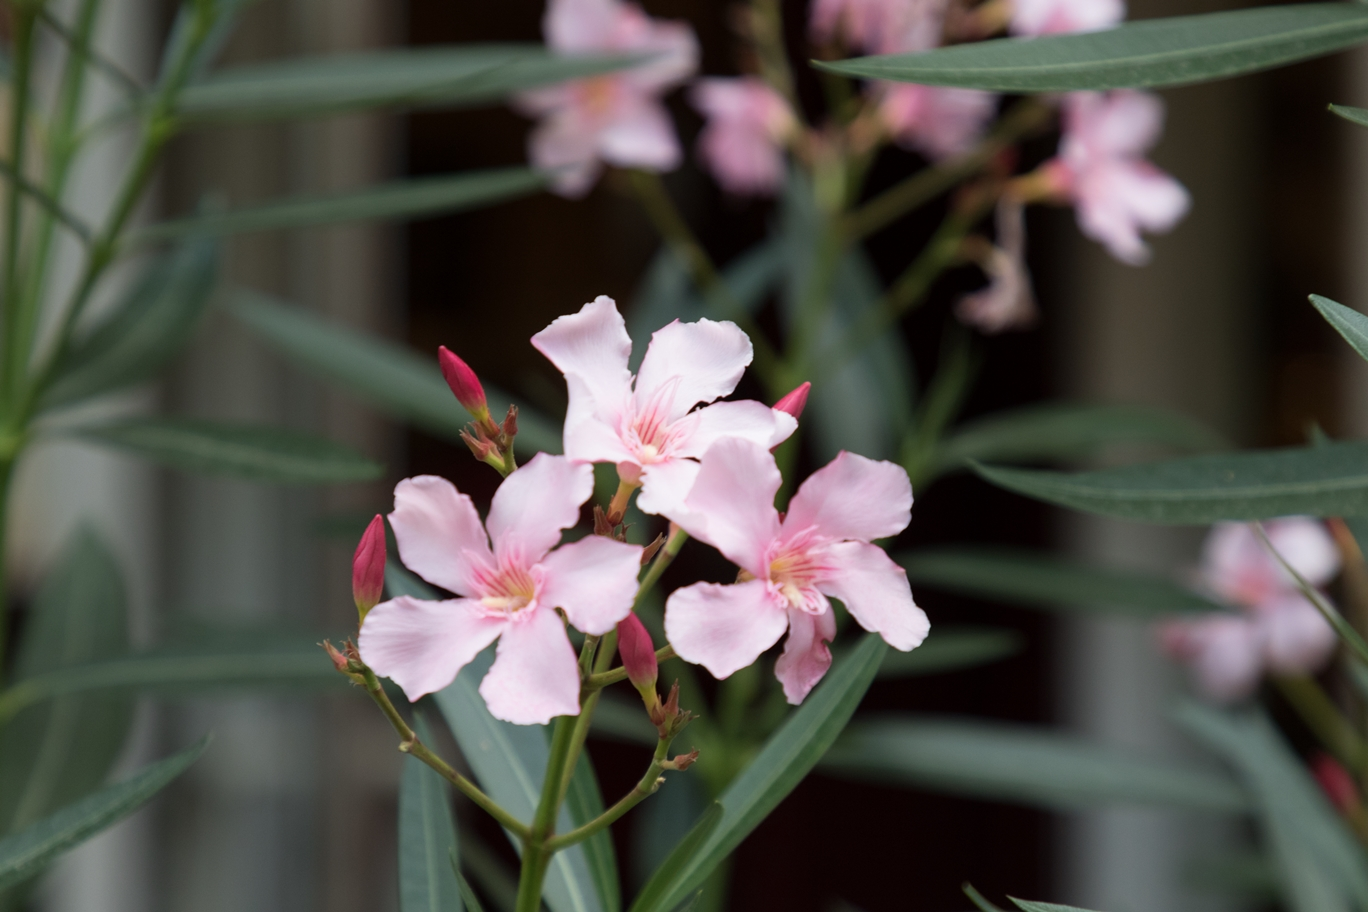
\includegraphics[width=0.4\textwidth]{resources/A3_compact.jpg}
        \caption{Original A3.png}
        \label{fig:a3_input}
    \end{figure}
    
    \begin{figure}[h]
        \centering
        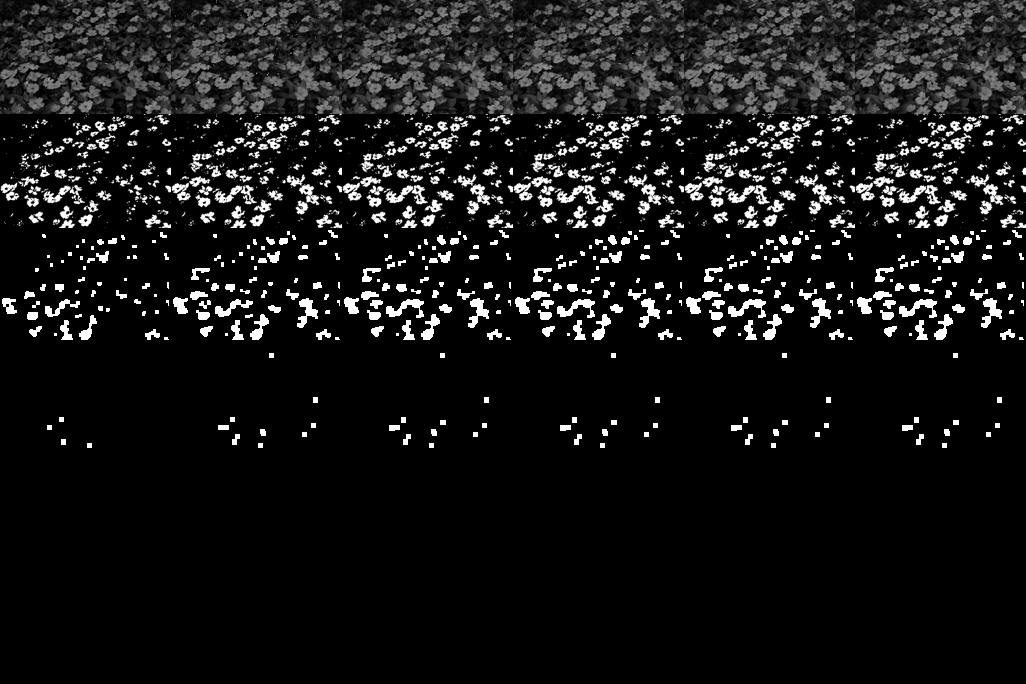
\includegraphics[width=0.4\textwidth]{resources/A1_compare.jpg}
        \caption{Different size of structuring elements as columns, gray-scale output of top hat operation, binarized version of the operation result, and different sizes of structuring elements used for cleaning the noise by opening and closing operations as its rows}
        \label{fig:a1_compare}
    \end{figure}

    \begin{figure}[h]
        \centering
        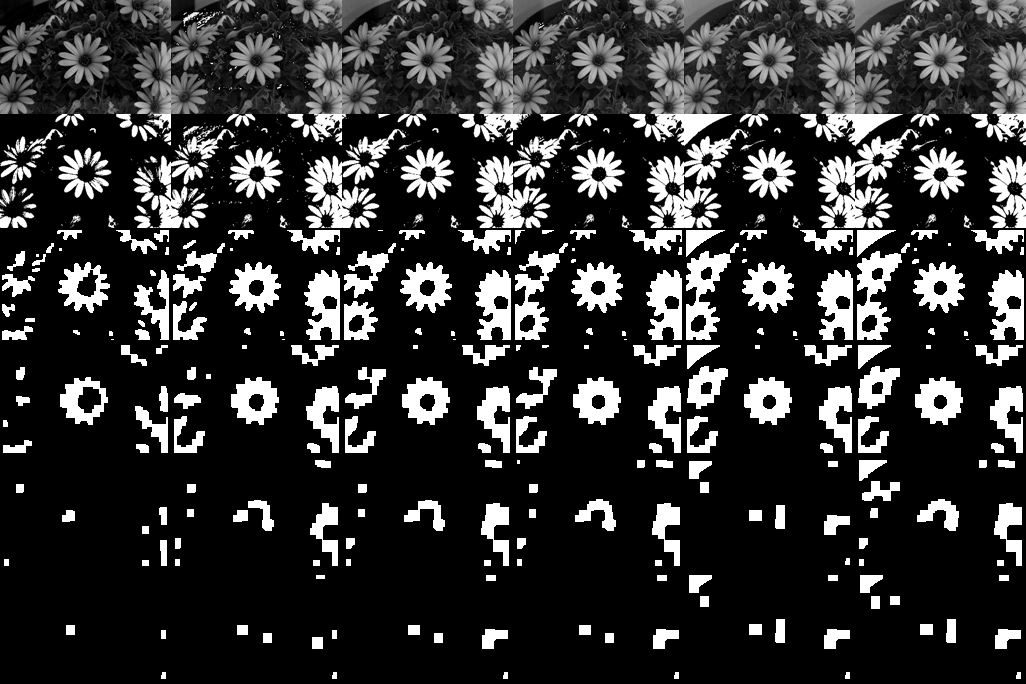
\includegraphics[width=0.4\textwidth]{resources/A2_compare.jpg}
        \caption{Different size of structuring elements as columns, gray-scale output of top hat operation, binarized version of the operation result, and different sizes of structuring elements used for cleaning the noise by opening and closing operations as its rows}
        \label{fig:a2_compare}
    \end{figure}

    \begin{figure}[h]
        \centering
        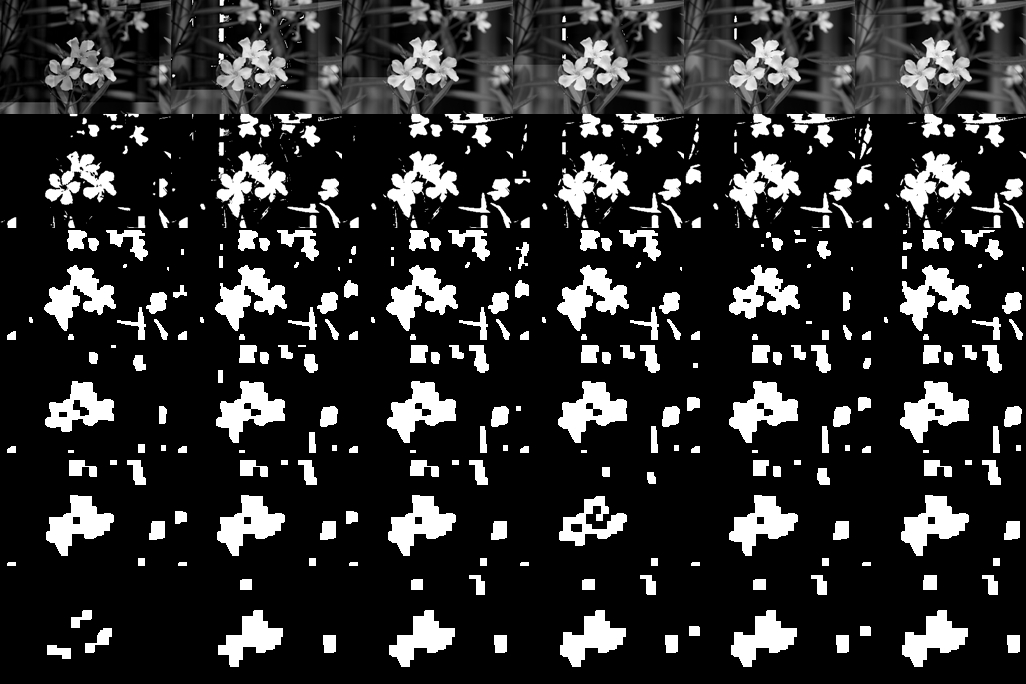
\includegraphics[width=0.4\textwidth]{resources/A3_compare.jpg}
        \caption{Different size of structuring elements as columns, gray-scale output of top hat operation, binarized version of the operation result, and different sizes of structuring elements used for cleaning the noise by opening and closing operations as its rows}
        \label{fig:a3_compare}
    \end{figure}

    Because mathematical morphology is limited to the gray-scale or binary images and our input images are 5472x3648 in dimensions, we start our process by first down-sampling our input images by a factor of 16, and then turned them to gray-scale by using their intensity value.

    Then, for object counting, we used top hat operation on the gray-scale image to detect objects. We had a variety of options when it comes to the size of the structuring element. We tested a many sizes for the element, all being square in shape. Results of different structuring elements can be seen in row 1 of Figures \ref{fig:a1_compare}, \ref{fig:a2_compare}, and \ref{fig:a3_compare}.

    After using top-hat operation, we binarized the images, using $I = 100$ as the threshold intensity value. We arrived at this threshold by examining the intensity values in the results of the morphological operation. Binarized outputs for different structuring elements can also be seen in Figures row 2 of \ref{fig:a1_compare}, \ref{fig:a2_compare}, and \ref{fig:a3_compare}. After binarization, we still had some amount of noise. To eliminate it, we decided to use opening and closing morphological operations on the binarized images. This once again introduced the design decision about the size of the structuring element. We once again tried a variety of options, results of which can be seen in rows 3, 4, 5, and 6 of Figures \ref{fig:a1_compare}, \ref{fig:a2_compare}, and \ref{fig:a3_compare}.

    After comparing different options we arrived at the values which turned the images at Figures \ref{fig:a1_input}, \ref{fig:a2_input}, and \ref{fig:a3_input} into Figures \ref{fig:a1_output}, \ref{fig:a2_output}, and \ref{fig:a3_output} with the object counts 53, 7, an 6. We had configurations which had more accurate object counts but they didn't counted the actual flowers and counted some amount of noise to compensate for the flowers they didn't count. We chose the configurations that were the most successful in both the accurate count and the ones that counted the flowers, as best as we could.

    \begin{figure}[h]
        \centering
        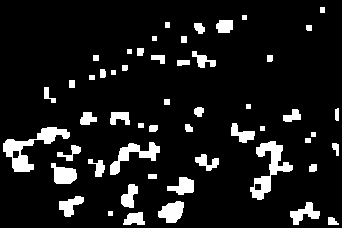
\includegraphics[width=0.4\textwidth]{resources/A1.png}
        \caption{Final A1.png}
        \label{fig:a1_output}
    \end{figure}
    \begin{figure}[h]
        \centering
        
\includegraphics[width=0.4\textwidth]{resources/A2.png}
        \caption{Final A2.png}
        \label{fig:a2_output}
    \end{figure}
    \begin{figure}[h]
        \centering
        
\includegraphics[width=0.4\textwidth]{resources/A3.png}
        \caption{Final A3.png}
        \label{fig:a3_output}
    \end{figure}

\section{Segmentation Algorithms}
Image segmentation is a very important topic that has usages spanning where there is some context based application. We had two algorithms to use in this assignment. Namely mean shift algorithm and n-cut algorithm. In both usages of these algorithms we pre-processed the images before feeding them to the algorithms. We applied median blurring to get rid of some of the noise from the image. We thought median filter would be better than an averaging filter due to median filter not increasing the number of different colors by using the existing ones. Than we used bit plane slicing to get rid of the last 4 bits of the 8 bit integer colors, this helped us deal with almost half the number of colors than the original and color palette's size is a factor in computation time. We lastly down sampled the images for faster computation time and more smoothing. It was exceptionally handy for large input images. 

\subsection{Mean Shift Algorithm}
Mean shift algorithms main idea is using rgb color values like coordinates on a 3d space and finding local maxima points. Mean shift algorithm starts by choosing a point and calculating local mean of points that are closer than a certain distance. After finding mean algorithm compares this mean value with the original point, if distance between them is more than a certain threshold we will shift the point. If the distance between new mean value and original point is less than the threshold we will say it is converged and jump to the next pixel. Why are we doing this? By following the closest mean we expect to gather all surrounding pixels to nearest local maxima and get a same colored region on the image. We have two important parameters while using this algorithm, first being the threshold and second being the radius of the area surrounding the chosen pixel. How does these effect the output;
\begin{itemize}
\item \textbf{Radius(Bandwidth):} Using a bigger radius means the algorithm will consider more points around the chosen pixel and at the output this will create smoother boundaries but this means increasing this value too much will cause loss on percision and make it harder to differanciate neighbouring regions. Algorithm we uses find the best bandwidth according to image's color values.
\item \textbf{Threshold:} Threshold effect the convergence time directly, smaller threshold means smaller changes will be counted and our algorithm will continue. Convergence time means more computation time but the results will be more accurate. 
\item \textbf{Cluster Size:} We can determine a minimum cluster size and eliminate clusters under this value by mapping them to the closest cluster. This will help us reduce the tiny clusters that cause noise on the output. 
\end{itemize}

Choosing these values is a matter of problem at hand, design choice. We can determine the best values for this by doing a grid search or via intuition. 

\begin{figure}[h]
        \centering
        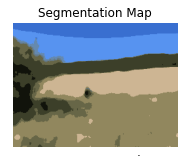
\includegraphics[width=0.4\textwidth]{resources/1_s.png}
        \caption{Segmentation output of mean shift algorithm by eliminating clusters that contain under 50 pixel using B4}
        \label{fig:1_s}
    \end{figure}

\begin{figure}[h]
        \centering
        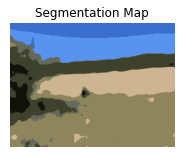
\includegraphics[width=0.4\textwidth]{resources/2_s.png}
        \caption{Segmentation output of mean shift algorithm by eliminating clusters that contain under 100 pixel using B4}
        \label{fig:2_s}
    \end{figure}

\begin{figure}[h]
        \centering 
        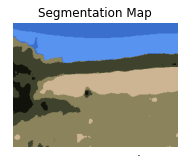
\includegraphics[width=0.4\textwidth]{resources/3_s.png}
        \caption{Boundary overlay output of mean shift algorithm by eliminating clusters that contain under 150 pixel using B4}
        \label{fig:3_s}
    \end{figure}

We can see the effects of this tiny clusters on our boundary overlay images too.

\begin{figure}[h]
        \centering
        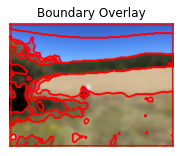
\includegraphics[width=0.4\textwidth]{resources/1_b.png}
        \caption{Boundary overlay output of mean shift algorithm by eliminating clusters that contain under 50 pixel using B4}
        \label{fig:1_b}
    \end{figure}

\begin{figure}[h]
        \centering
        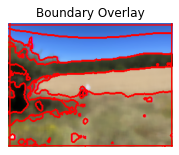
\includegraphics[width=0.4\textwidth]{resources/2_b.png}
        \caption{Boundary overlay output of mean shift algorithm by eliminating clusters that contain under 100 pixel using B4}
        \label{fig:2_b}
    \end{figure}

\begin{figure}[h]
        \centering 
        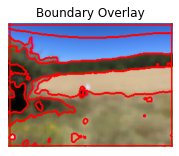
\includegraphics[width=0.4\textwidth]{resources/3_b.png}
        \caption{Boundary overlay output of mean shift algorithm by eliminating clusters that contain under 150 pixel using B4}
        \label{fig:3_b}
    \end{figure}

The image with the cluster with size under 150 has cleaner boundaries. 

\subsection{N-cut Algorithm}
\textbf{BEWARE: } N-cut algorithm we use does not work with the same version that is needed for the $networkx$ library. N-cut only works with the version 2.6.3 of networkx and networkx works with only the latest release. We still got the both outputs by using different environments but there was no way we could think of for getting the graph and tree representations of the n-cut segmentation outputs. Coding was really similar, getting the labels for the segmentations of image through algortihms and representing part was the same. We still put the n-cut segmentation code to the end so there should not be any problems with the other parts of the code.
\textbf{BEWARE END}

N-cut algorithm is basically a graph partioning algorithm with a goal that is minimizing the weights between partionings and maximizing the weights inside the partionings. N-cut algorithms outputs were sharper than mean shift algorithm's, mean shift detected the color differences on big objects as boundaries. But mean shift algorithm's outputs were more accurate when it could detect the edges. This is due to mean shift algorithm using only color information but n-cut segmentation using both color and spacial distance values.

When using n-cut algorithm we can change the weights of color values or spacial distance values effect on the edge values we try to minimize or maximize. Algorithm we used gave us the option to change how many clusters we wanted. Here are some examples with different values of this parameter;

\begin{figure}[h]
        \centering
        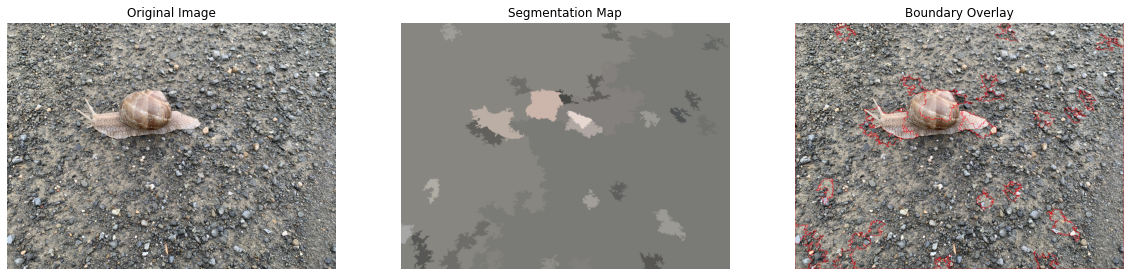
\includegraphics[width=0.4\textwidth]{resources/snail_1.png}
        \caption{Boundary overlay and segmentation outputs of n-cut algorithm by using image B1 and $n_segments$ parameter as 200}
        \label{fig:snail_1}
    \end{figure}

\begin{figure}[h]
        \centering
        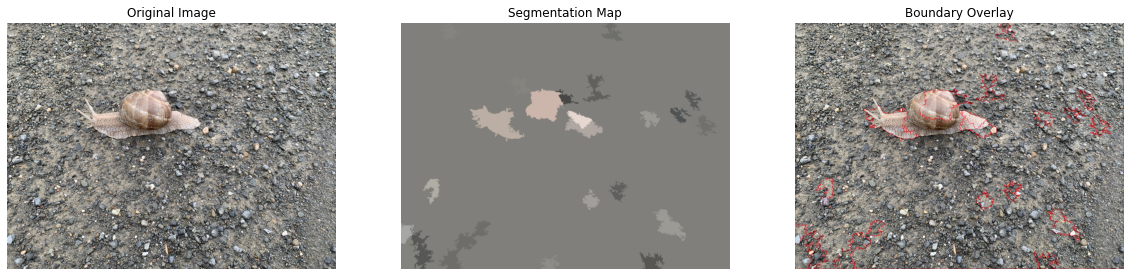
\includegraphics[width=0.4\textwidth]{resources/snail_2.png}
        \caption{Boundary overlay and segmentation outputs of n-cut algorithm by using image B1 and $n_segments$ parameter as 400}
        \label{fig:snail_2}
    \end{figure}

\begin{figure}[h]
        \centering 
        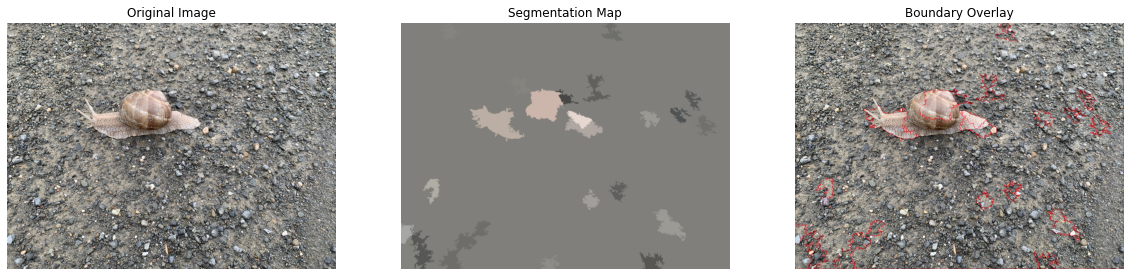
\includegraphics[width=0.4\textwidth]{resources/snail_3.png}
        \caption{Boundary overlay and segmentation outputs of n-cut algorithm by using image B1 and $n_segments$ parameter as 600}
        \label{fig:snail_3}
    \end{figure}

Values we tried turned out to be too big to have a detectible change especially between 400 and 600. But we can still see that there is a line in the middle of the picture that separates the shady part of the ground from the sunny part. Increasing this parameter means increasing the cluster number and this means more detailed segmentations.

\subsection{Representations of the segmented images}
Main reason of segmentation is getting the possible objects, backgrounds or parts of the objects separatey.  After this we may want to look at the realationships between these segments to get a sensei some information about the context. To see more clearly and use these relations we may want to represent/visualize them in different ways. For this assignment we had two options. A region adjacency graph or a relation tree structure. Region adjacency graphs give us information about which regions are neighbours/touching each other and relation tree give information about what are the main components of the image and if there is what do they contain.

\begin{figure}[h]
        \centering
        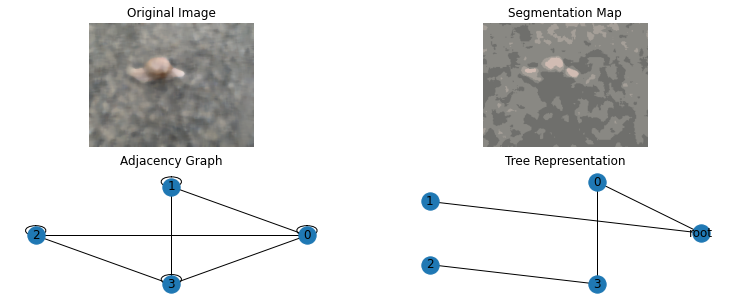
\includegraphics[width=0.4\textwidth]{resources/r_1.png}
        \caption{Original image, segmentation map, graph representation and tree representation of the image B1}
        \label{fig:r_1}
    \end{figure}

\begin{figure}[h]
        \centering 
        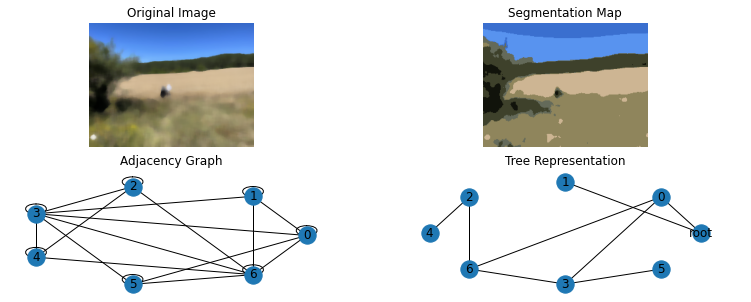
\includegraphics[width=0.4\textwidth]{resources/r_2.png}
        \caption{Original image, segmentation map, graph representation and tree representation of the image B4}
        \label{fig:r_2}
    \end{figure}

Especially on the second figure we can see that graph is almost like made out of two smaller and denser graphs. We might say that this image can be separated into two more connected, almost independent regions. 
And yes we can see that separating the original image as sky and ground would not be that wrong. 

From the tree relation we can say that this image' components/segments are more connected to one segment and there are lone segments too and yes again there is a lonely sky segment and more crowded ground segment in the image.

\section{Dependencies}
We used following libraries for the described reasons.
\begin{itemize}
	\item \textbf{os:} Handling non-existent input or output paths.
	\item \textbf{numpy:} Executing array and matrix operations.
	\item \textbf{PIL:} Reading images and converting them to arrays.
	\item \textbf{mathplotlib:} Writing arrays as image files.
    \item \textbf{sklearn:} Using MeanShift method and estimate\_bandwidth methods
    \item \textbf{networkx:} Creating graphs and trees
    \item \textbf{skimage:} Implementing n-cut segmentation
        
\end{itemize}

\end{document}
